\documentclass[12pt]{article}%
\usepackage{amsfonts}
\usepackage{fancyhdr}
\usepackage{comment}
\usepackage[a4paper, top=2.5cm, bottom=2.5cm, left=2.2cm, right=2.2cm]%
{geometry}
\usepackage{times}
\usepackage{amsmath}
\usepackage{changepage}
\usepackage{amssymb}
\usepackage{graphicx}
\usepackage{url}%
\setcounter{MaxMatrixCols}{30}
\newtheorem{theorem}{Theorem}
\newtheorem{acknowledgement}[theorem]{Acknowledgement}
\newtheorem{algorithm}[theorem]{Algorithm}
\newtheorem{axiom}{Axiom}
\newtheorem{case}[theorem]{Case}
\newtheorem{claim}[theorem]{Claim}
\newtheorem{conclusion}[theorem]{Conclusion}
\newtheorem{condition}[theorem]{Condition}
\newtheorem{conjecture}[theorem]{Conjecture}
\newtheorem{corollary}[theorem]{Corollary}
\newtheorem{criterion}[theorem]{Criterion}
\newtheorem{definition}[theorem]{Definition}
\newtheorem{example}[theorem]{Example}
\newtheorem{exercise}[theorem]{Exercise}
\newtheorem{lemma}[theorem]{Lemma}
\newtheorem{notation}[theorem]{Notation}
\newtheorem{problem}[theorem]{Problem}
\newtheorem{proposition}[theorem]{Proposition}
\newtheorem{remark}[theorem]{Remark}
\newtheorem{solution}[theorem]{Solution}
\newtheorem{summary}[theorem]{Summary}
\newenvironment{proof}[1][Proof]{\textbf{#1.} }{\ \rule{0.5em}{0.5em}}

\newcommand{\Q}{\mathbb{Q}}
\newcommand{\R}{\mathbb{R}}
\newcommand{\C}{\mathbb{C}}
\newcommand{\Z}{\mathbb{Z}}

\begin{document}

\title{CS280 Spring 2024 Assignment 1 \\ Part A}
\author{Basics \& MLP}
\maketitle

\paragraph{Name:}

\paragraph{Student ID:}

\newpage

\subsubsection*{1. \textit{Loss Function} (10 points).}

Generally speaking, a classifier can be written as $H(x) = sign(F(x))$, where $H(x):\mathbb{R}^d \rightarrow \{-1, 1\}$ and $F(x): \mathbb{R}^d \rightarrow \mathbb{R}$. To obtain the parameters in $F(x)$, we need to minimize the loss function averaged over the training set: ${\textstyle \sum_{i}^{}}L(y^iF(x^i))$. Here $L$ is a function of $yF(x)$. For example, for linear classifiers, $F(x)=w_0 + {\textstyle \sum_{j=1}^{d}}w_jx_j$, and $yF(x) = y(w_0 + {\textstyle \sum_{j=1}^{d}}w_jx_j)$.
\vspace{1em}
\\
(a) Which loss functions below are appropriate to use in classification? For the ones that are not appropriate, explain why not. In general, what conditions does $L$ have to satisfy in order to be an appropriate loss function? The x axis is $yF(x)$, and the y axis is $L(yF(x))$.
\begin{figure}[htpb]
    \centering
    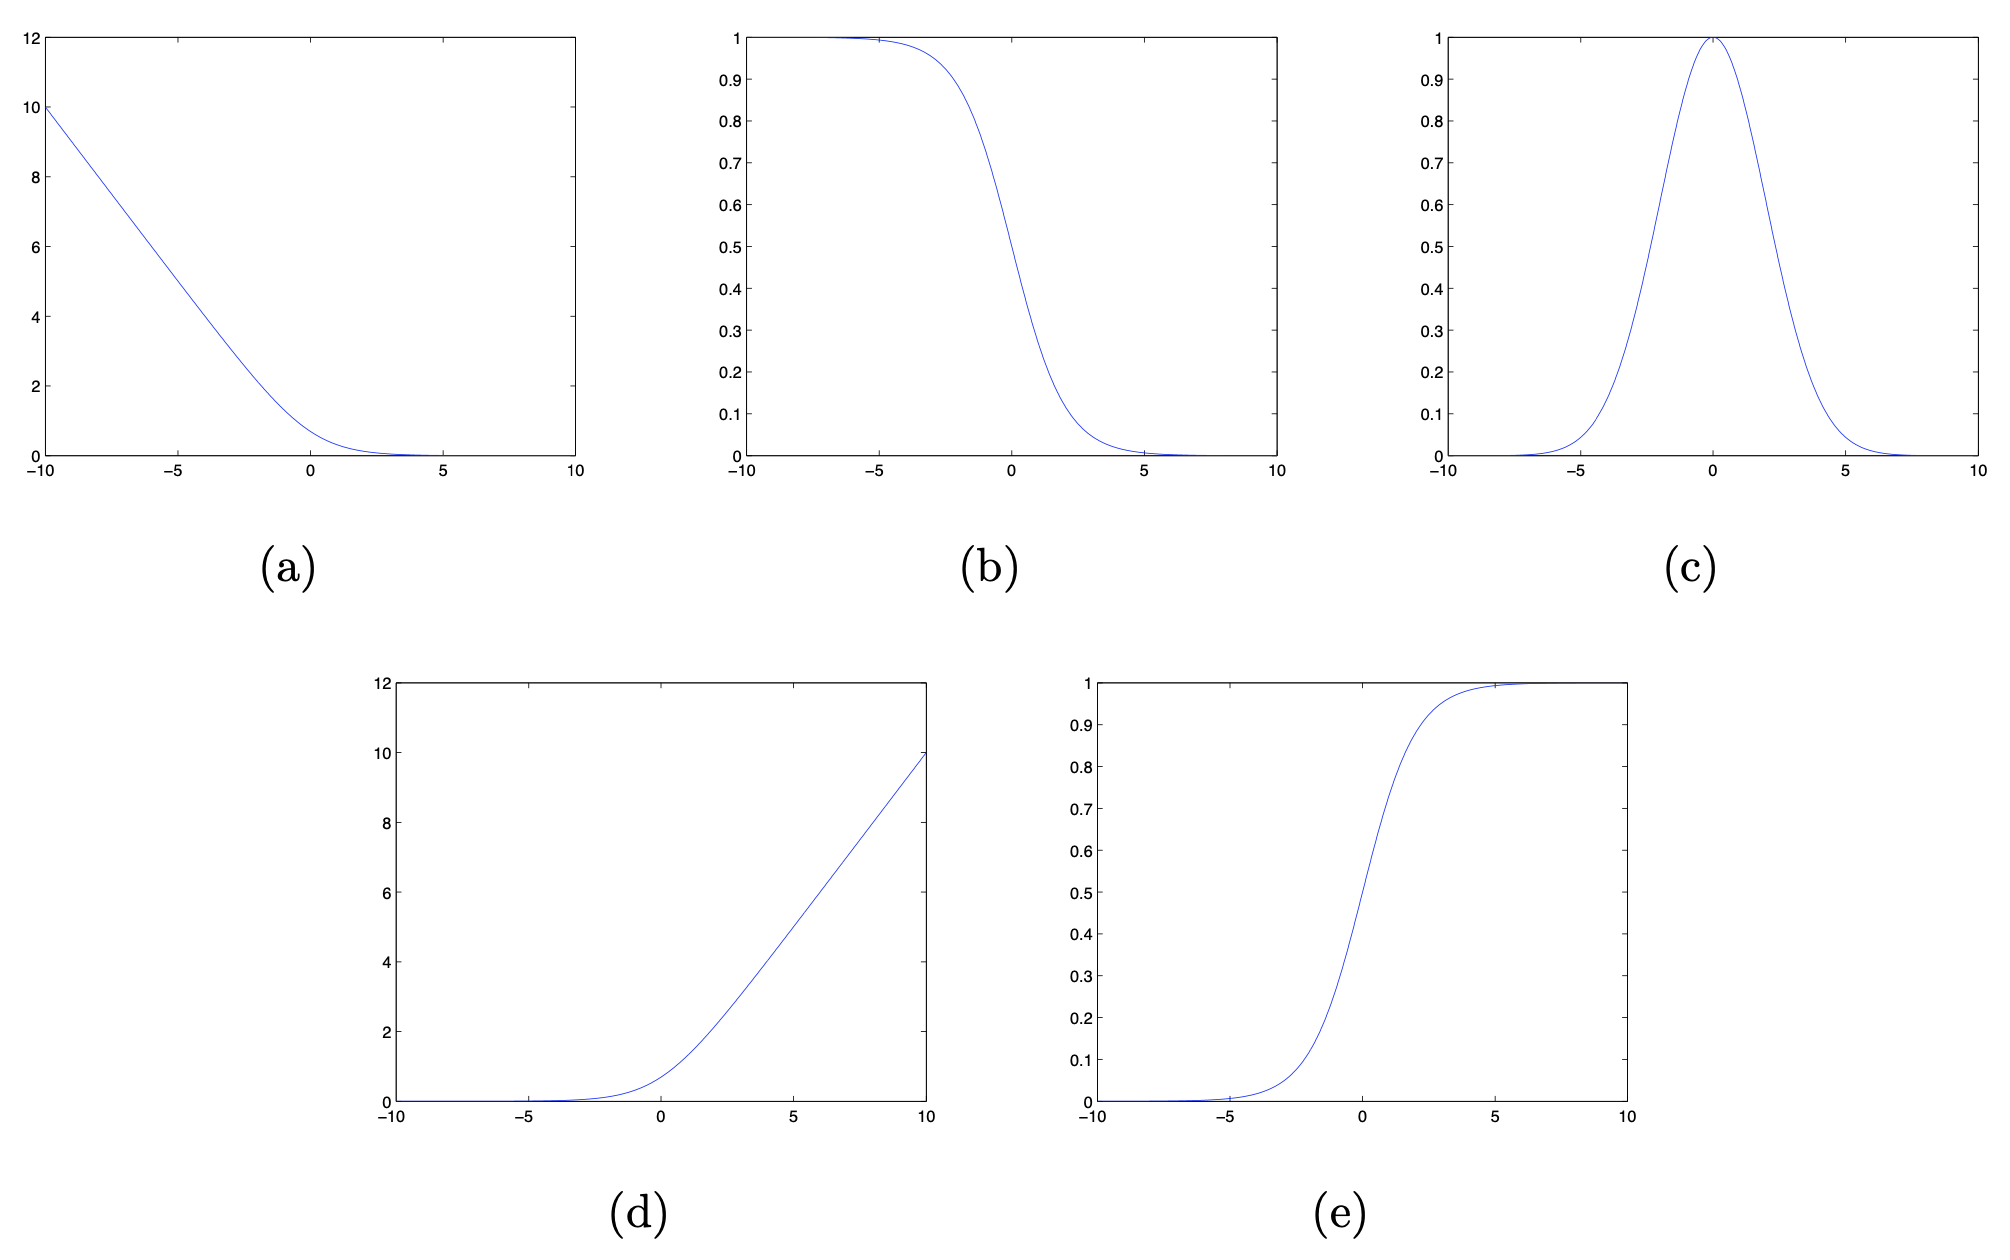
\includegraphics[scale=0.45]{partA_loss.png}
    \label{fig:enter-label}
\end{figure}
\vspace{1em}
\\
(b) Of the above loss functions appropriate to use in classification, which one is the most robust to outliers? Justify your answer.
\vspace{1em}
\\
(c) Let $F(x)=w_0+\sum_{j=1}^{d}w_jx_j$ and $L(yF(x))= \frac{1}{1+exp(yF(x))} $. Suppose you use gradient descent to obtain the optimal parameters $w_0$ and $w_j$. Give the update rules for these parameters.

\pagebreak

\subsubsection*{2. \textit{Sotfmax \& Computation Graph} (10 points).}
Recall that the softmax function takes in a vector $(z_1, \dots , z_D)$ and returns a
vector $(y_1, \dots , y_D)$. We can express it in the following form:
\begin{equation*}
    \begin{split}
    r = \sum_j e^{z_j}   \qquad y = \frac{e^{z_j}}{r}
\end{split}
\end{equation*}
(a) Consider $D = 2$, i.e. just two inputs and outputs to the softmax. Draw the
computation graph relating $z_1$, $z_2$, $r$, $y_1$, and $y_2$.
\vspace{1em}
\\
(b) Determine the backprop updates for computing the $\bar{z_j}$ when given the $\bar{y_i}$.
You need to justify your answer. (You may give your answer either for
$D = 2$ or for the more general case.)
\vspace{1em}
\\
(c) Write a function to implement the vector-Jacobian product (VJP) for the
softmax function based on your answer from part (b). For efficiency, it should
operate on a mini-batch.
The inputs are:
\begin{itemize}
    \item a matrix \textit{\textbf{Z}} of size $N \times D$ giving a batch of input vectors. $N$ is the batch
size and $D$ is the number of dimensions. Each row gives one input vector
$z = (z_1, \dots , z_D)$.
    \item A matrix $\mathbf{Y_{bar}}$ giving the output error signals. It is also $N \times D$
\end{itemize} 
\indent The output should be the error signal $\mathbf{Z_{bar}}$. Do not use a for loop.
\end{document}